\chapter{Diffusion Models}
\label{ch:03-diffusion-models}

\lecturemeta{Sander Dieleman}{Google DeepMind}

Diffusion is one of two ways to break generation into easy steps, and almost every design
decision people argue about turns out to be downstream of a single equation for the forward
corruption process. Once
$\xt = \alpha(t)\xz + \sigma(t)\eps$ is on the board, the variance-preserving,
variance-exploding and flow-matching families are three choices of $\alpha$; predicting
$\xz$, $\eps$ or a velocity are interconvertible parameterisations of one object; guidance
is Bayes' rule applied to the score; and the question of why diffusion works so well on
images has a spectral answer that Dieleman states as a slogan. The final third is about
where the framework strains: distillation, discrete data, and what a latent space is for.

\section*{Key ideas}

\paragraph{Two roads to iterative refinement, and the space matters more than the road.}
Iterative refinement breaks the generative procedure into simpler steps in which all steps
are of comparable difficulty. Autoregression does this with the chain rule of probability,
$p(\xin) = \prod_i p(\xin_i \given \xin_{<i})$, and Dieleman's historical sequence makes the
point that the interesting variation was never the factorisation but the space it acts on:
pixels in PixelRNN and PixelCNN~\citep{oord2016pixelrnn}, raw amplitudes in
WaveNet~\citep{oord2016wavenet}, discrete latents in VQ-VAE~\citep{oord2017vqvae}. Diffusion
factorises differently, by iterative denoising, and the same lesson applies: production
systems run diffusion in a latent space, not in pixels, compressing a $3 \times 256 \times
256$ image to something like $8 \times 32 \times 32$ before the diffusion model ever sees
it.\footnote{This is the point the personal notes flag as ``Diffusion is done in latent
space, not in pixel space!''. The deck supports it with a pixels-versus-latents slide and a
pointer to regularising the latent space for generative modelling.}

\begin{figure}[htbp]
\centering
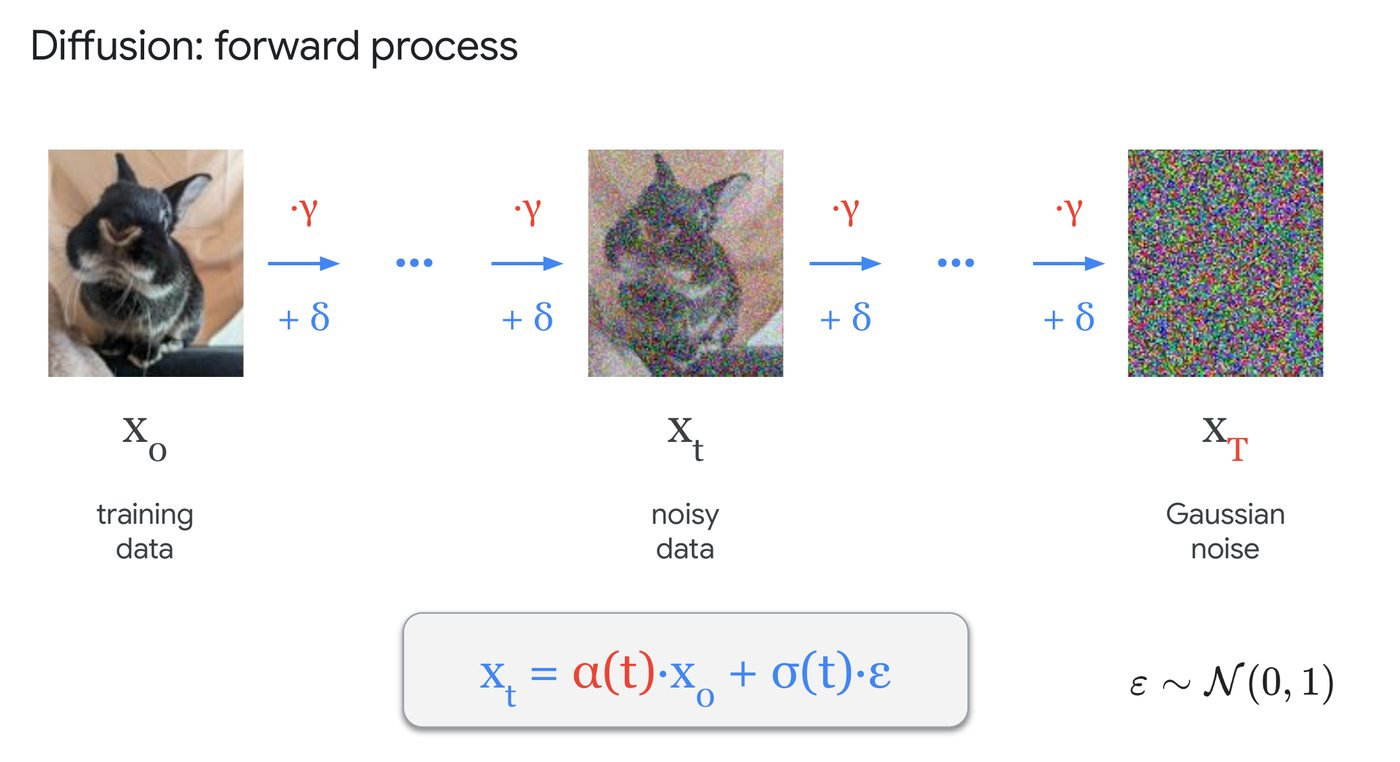
\includegraphics[width=0.82\textwidth]{figures/diffusion-models-1.jpg}
\caption{The forward process, from the Diffusion Models lecture. Each step scales by
$\gamma$ and adds noise $\delta$, carrying training data $\xz$ through noisy data $\xt$ to
pure Gaussian noise $\vect{x}_T$. The whole chain collapses to the boxed line,
$\xt = \alpha(t)\xz + \sigma(t)\eps$: corruption is just an interpolation between the data
and a sample of noise.}
\label{fig:diffusion-models-1}
\end{figure}

\paragraph{One equation for the forward process.} Corruption interpolates between data and
noise (Figure~\ref{fig:diffusion-models-1}),
\[
  \xt = \alpha(t)\,\xz + \sigma(t)\,\eps,
  \qquad \eps \dist \Normal(\vect{0}, \id),
\]
\noindent where $\sigma(t)$ is the noise schedule controlling the rate of corruption. The
families differ only in $\alpha$: variance-preserving takes
$\alpha = \sqrt{1 - \sigma^2}$, variance-exploding takes $\alpha = 1$, and rectified flow or
flow matching takes $\alpha = 1 - \sigma$. Presented this way, a literature that usually reads as three
separate methods collapses into one line with a parameter.

\paragraph{What the network predicts is a free choice.} Since $\xt$ is a linear combination
of $\xz$ and $\eps$, a prediction of one converts into a prediction of the other, so
$\xz$-prediction, $\eps$-prediction, $v$-prediction with
$v = \alpha(t)\eps - \sigma(t)\xz$~\citep{salimans2022}, and the flow-matching target
$\eps - \xz$~\citep{lipman2022} are reparameterisations rather than different models. The
same object appears again as the score $\grad_{\xin} \log p(\xin)$, which points toward
regions of high density, so knowing the gradient is knowing
$p$~\citep{hyvarinen2005, vincent2011}. In practice all of these are trained by minimising a
mean squared error.

\paragraph{Guidance is Bayes' rule, twice.} Dieleman's own phrase, and the one the personal notes
record, is that guidance is ``a cheat code'': it buys sample quality at the cost of
diversity. Classifier guidance is derived on the slide straight from Bayes' rule, in three
lines:
\[
\begin{aligned}
  p(\xin \given c) &\propto p(c \given \xin)\, p(\xin), \\
  \log p(\xin \given c) &= \log p(c \given \xin) + \log p(\xin) + C, \\
  \underbrace{\grad_{\xin} \log p(\xin \given c)}_{\text{conditional score}}
    &= \underbrace{\grad_{\xin} \log p(c \given \xin)}_{\text{classifier gradient}}
     + \underbrace{\grad_{\xin} \log p(\xin)}_{\text{unconditional score}}.
\end{aligned}
\]
\noindent The normalising constant differentiates away, which is the whole trick: the
conditional score is the unconditional score plus a classifier gradient, so an unconditional
model becomes conditional without retraining. A
scale factor $\guide$ on the second term acts as an inverse temperature, and the lecture is
careful about what it sharpens: it sharpens $p(c \given \xin)$, which is not the same thing
as sharpening $p(\xin)$ or $p(\xin \given c)$. Classifier-free guidance drops the separate
classifier: predict $\est{\xz}$ and $\est{\xz}_{|c}$ from one model trained with conditioning
dropout, take the difference $\delta$, and amplify it by $\guide$. The insight is that
$\delta$ is itself a Bayesian classifier, so this is Bayes' rule applied twice, and it is
less prone to adversarial examples than guiding with a real
classifier~\citep{nichol2022glide}. Figure~\ref{fig:diffusion-models-2} shows guidance as a geometric
operation on one sampling step, not a change to the model.

\begin{figure}[htbp]
\centering
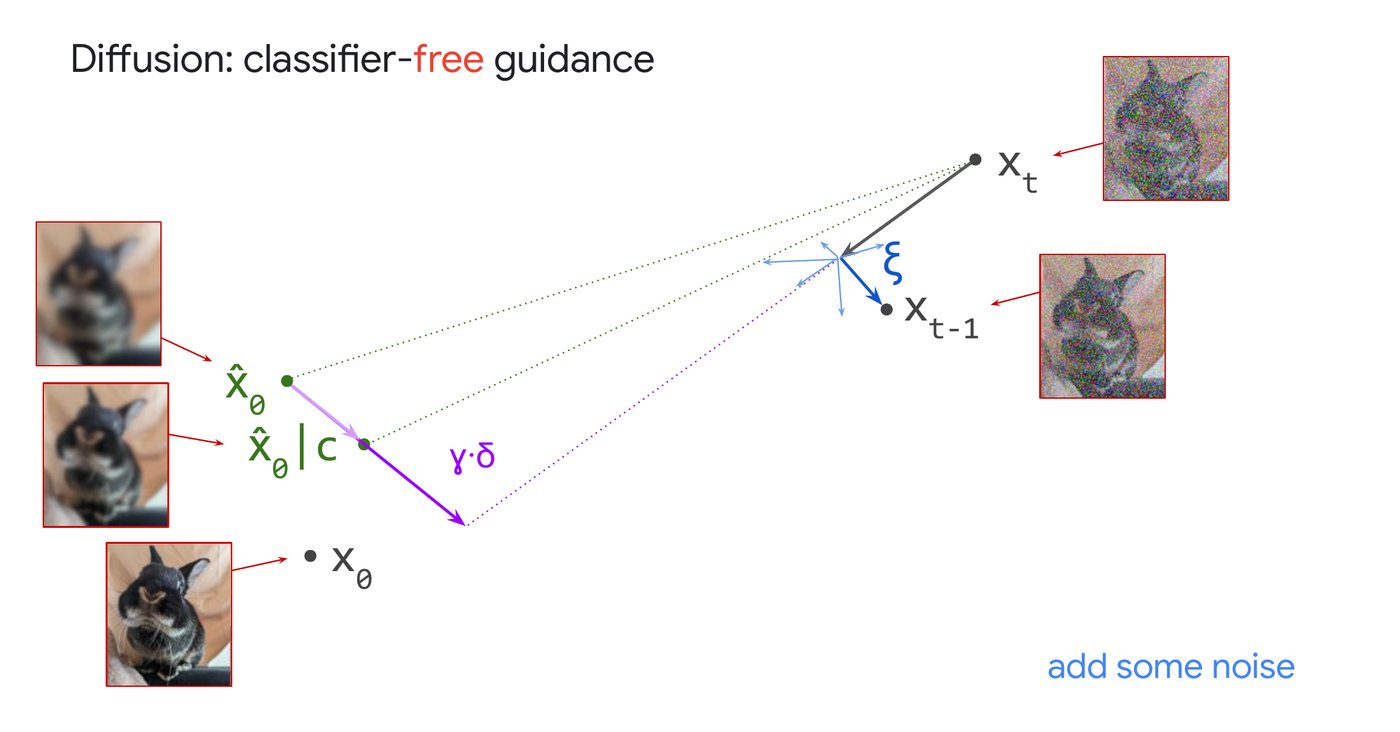
\includegraphics[width=0.86\textwidth]{figures/diffusion-models-2.jpg}
\caption{Classifier-free guidance as one sampling step, from the Diffusion Models lecture.
From the noisy state $\xt$ the model predicts both an unconditional $\est{\xz}$ and a
conditional $\est{\xz}_{|c}$; their difference $\delta$ is scaled by $\gamma$ and
extrapolated past the conditional prediction, then a small step is taken toward that
extrapolated target and fresh noise $\xi$ is added to reach $\vect{x}_{t-1}$. Note that the
guided target overshoots $\xz$ entirely, which is exactly why guidance trades diversity for
apparent quality.}
\label{fig:diffusion-models-2}
\end{figure}

\paragraph{Diffusion is approximate spectral autoregression.} The lecture's answer to why
diffusion works so well on images is spectral, and it is the insight the personal notes single out.
Natural images have a power spectrum that falls off steeply with spatial frequency, while
Gaussian noise is flat. Adding noise at level $\sigma$ therefore does not damage all scales
equally: it drowns everything above the frequency where the flat noise floor crosses the
image's decaying spectrum, and leaves the low frequencies almost intact
(Figure~\ref{fig:diffusion-models-3}). Sampling, run backwards, is then recovering
frequency bands roughly coarsest-first, which is why Dieleman puts it as diffusion being
approximate spectral autoregression~\citep{dieleman2023perspectives}. It also explains why
the trick transfers poorly to data without a decaying spectrum.

\begin{figure}[htbp]
\centering
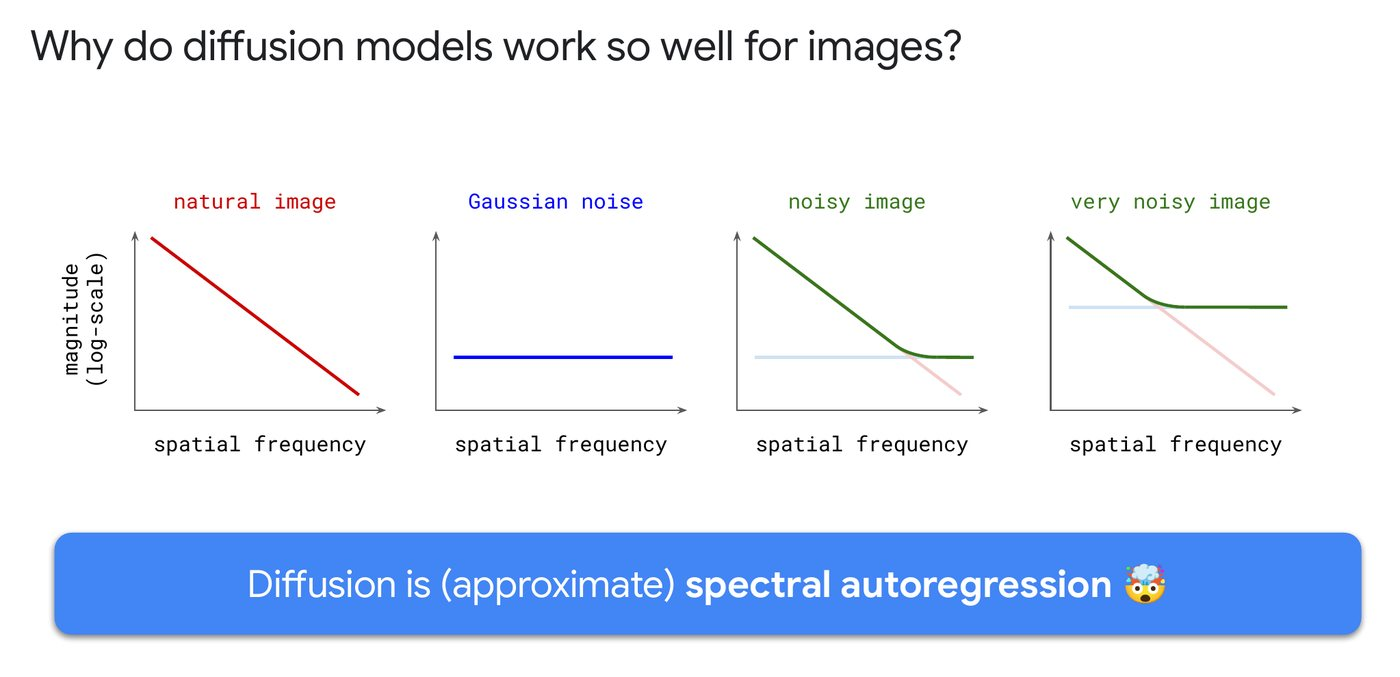
\includegraphics[width=0.88\textwidth]{figures/diffusion-models-3.jpg}
\caption{The spectral argument, from the Diffusion Models lecture. A natural image's
magnitude spectrum falls steeply with spatial frequency while Gaussian noise is flat, so
their sum is the pointwise maximum: at moderate noise the high frequencies are already
replaced by the noise floor, and at high noise only the lowest frequencies survive. Read
right to left, sampling restores frequency bands coarsest-first, which is the sense in which
diffusion is approximate spectral autoregression.}
\label{fig:diffusion-models-3}
\end{figure}

\paragraph{Where the framework strains.} Three limitations close the lecture.
Distillation into fewer sampling steps requires cutting corners, and the corners are entropy
and diversity first, then visual fidelity~\citep{dieleman2024paradox, song2023consistency}.
Discrete data breaks the score outright, since $\grad_{\xin} \log p(\xin)$ is undefined when
$\xin$ is discrete; the two escapes are to define a discrete corruption process, or to embed
the data in a continuous space, which is what CDCD does while deliberately making diffusion
look familiar to language-model practitioners by using an unmasked Transformer and a
cross-entropy loss instead of an MSE~\citep{dieleman2022cdcd}. And data curation is named as
essential for high-quality results while being structurally disincentivised in the research
community.

\section*{Notation}

$\xz$ is clean data, $\xt$ the corrupted state at time $t$, $\eps$ standard Gaussian noise,
$\alpha(t)$ and $\sigma(t)$ the interpolation coefficients, and $\guide$ the guidance scale.
The deck writes the guidance scale as a Greek gamma. It is $\guide$ here, to keep it clear of the
discount factor in Chapter~\ref{ch:04-intro-reinforcement-learning}.

\section*{Why it matters}

The parameterisation argument travels furthest. Whenever a literature presents $n$ competing
methods, ask whether they are $n$ choices of one coefficient.
The spectral analysis connects directly to Stanković's lecture
(Chapter~\ref{ch:09-spectral-analysis-dags}), which also treats a spectrum as the object to
manipulate, though on graphs rather than grids, and to Veličković's argument
(Chapter~\ref{ch:11-geometric-deep-learning}) that the structure of the data domain should
dictate the model. Classifier-free guidance reappears in the summer school's
multimodal tutorial, where it is the single line the notebook asks to be written by hand.

\begin{aside}
Two threads to pull. The personal notes record the claim that diffusion models are
essentially RNNs, which permits training much deeper networks. That framing is not on the
slides in those words, though it is consistent with the iterative-refinement picture where
one network is applied repeatedly with a time input; treat it as a remark from the room
rather than a slide. Second, the deck's closing list of untouched topics includes flow maps,
also flagged in the personal notes, pointing at Dieleman's blog~\citep{dieleman2026flowmaps}. That
is the natural continuation of the unification of diffusion and flow matching set out above.
\end{aside}
